\chapter{Problem Formulation}\label{ch:problem_formulation}

This chapter systematically formulates the targetted task of robotic grasping as an MDP, while describing the applied reward function alongside the utilised observation and action spaces. The corresponding implementation of such formulation with detailed specifications is covered in the next chapter \autoref{ch:implementation}.

In this work, the agent is assumed to be a high-level controller that provides sequential decision making in form of gripper poses and actions. Therefore, the environment is considered to not only include all objects and the physical interactions between them but also the robot with its actuators and low-level controllers. Episodic formulation of the grasping task is studied in this work, where a new set of objects is introduced into the scene at the beginning of each episode when the environment is reset. During each episode, the aim of the agent is to grasp and lift an object certain height above the ground plane that the objects rest on, which also terminates the current episode. Furthermore, an episode is also terminated after a fixed number of time steps and whenever the agent pushes all objects outside the union of the perceived and reachable workspace. Placing of objects after their picking is not investigated in this work.

Due to the benefits of employing robotics simulators to train RL agents, e.g. safe and inexpensive data collection, robotics simulator will be used in this work to train the agent. Once the agent is trained in a virtual environment, the learned policy will subsequently be evaluated in a real-world setup via sim-to-real transfer. The conceptual setup of this work that should be similar in both domains is illustrated in \autoref{fig:problem_formulation_setup_sketch}.

\begin{figure}[ht]
    \centering
    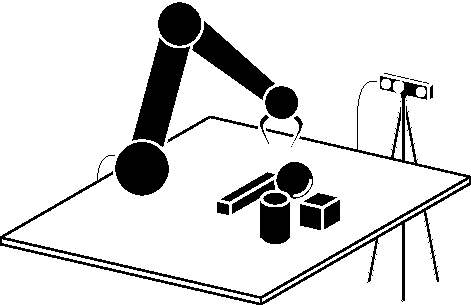
\includegraphics[width=0.667\textwidth]{problem_formulation/setup_sketch.pdf}
    \caption{Conceptual setup for the task of robotic grasping that needs to be constructed both inside a robotics simulator for training and in real-world domain for subsequent evaluation. The goal of the RL agent is to grasp and lift any object from the scene that is perceived by a statically mounted RGB-D camera.}
    \label{fig:problem_formulation_setup_sketch}
\end{figure}


\section{Observation Space}

The observation space for the grasping task used in this work comprises of visual and proprioceptive observations. Furthermore, a number of sequential observations is stacked together for each transition in order to provide the agent with temporal information about environment states.


\subsection{Octree}

The visual observations utilised in this work are represented in form of 3D octrees. As already mentioned, the visual perception originates from a statically mounted RGB-D camera, which is assumed to provide a new RGB image and depth map of the scene at each time step. Before constructing an octree, the depth map is first used to create a point cloud of the scene as an intermediate representation. This point cloud is colourised with a corresponding RGB image that is registered to the optical frame of the camera's depth sensor. Therefore, the resulting point cloud is in form of an unstructured list of \((x,y,z,r,g,b)\) tuples that represent individual points.

Hereafter, three assumptions about the use of volumetric 3D data representation for end-to-end robotic manipulation are set forth. First, aspect ratio of~1:1:1 is considered to provide generalisation over all possible directions of movement, i.e.~traversing a fixed distance along any of the primary axes should result in a movement over the same number of cells. Second assumption considers the volume that each cell occupies, which shall remain fixed over the entire duration of training and evaluation. This is considered to be beneficial because fixed scale of cells provides a consistency over distances between any two cells. Lastly, each cell should correspond to a specific position of space that remains fixed with respect to the robot pose, regardless of the camera pose. This assumption is considered to be necessary as it allows NNs to create relations among individual cells and their significance in space.

Due on these assumptions, the approach that is commonly used in classification and segmentation tasks, i.e.~rescale a point cloud to fit inside a fixed volume \cite{wang_o-cnn_2017}, cannot be applied in this work. However, it is assumed that the relative pose of camera with respect to robot is known, e.g.~through calibration process, therefore, the previously obtained point cloud is transformed into the robot coordinate frame in order to achieve invariance to camera pose. Furthermore, such point cloud is subsequently cropped in order to occupy a fixed volume in space with aspect ratio of~1:1:1. This volume is considered to be the observed workspace and it is subsequently used to construct the octree observations as illustrated in \autoref{fig:problem_formulation_octree_creation_sketch}. 

\begin{figure}[ht]
    \centering
    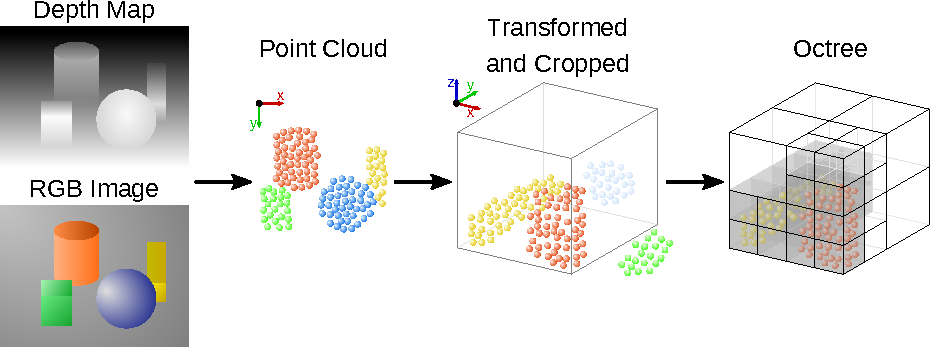
\includegraphics[width=\textwidth]{problem_formulation/octree_creation_sketch.pdf}
    \caption{Process of constructing an octree from depth map and RGB image via an intermediate point cloud, which is transformed into the robot coordinate frame and cropped to a fixed volume.}
    \label{fig:problem_formulation_octree_creation_sketch}
\end{figure}




\subsection{Proprioceptive Observations}


\subsection{Observation Stacking}



\section{Action Space}

% Mention this here
% Some problems are better solved with other traditional method instead of RL. (when talking about control of joint vs cartesian pose)


\section{Reward Function}



\section{Curriculum and Demonstrations}


